\documentclass[10pt,conference]{IEEEtran}

\usepackage[T1]{fontenc}
\usepackage{times}
\usepackage{amsmath,amssymb,amsfonts}
\usepackage{booktabs}
\usepackage{graphicx}
\usepackage[caption=false,font=footnotesize]{subfig}
\usepackage{algorithm}
\usepackage{algpseudocode}
\usepackage{xcolor}
\usepackage{cite}
\usepackage{url}

\newcommand{\WPRO}{\textsc{WPRO}}
\newcommand{\calW}{\mathcal{W}}
\newcommand{\calR}{\mathcal{R}}
\newcommand{\calG}{\mathcal{G}}
\newcommand{\calM}{\mathcal{M}}
\newcommand{\calA}{\mathcal{A}}
\newcommand{\calV}{\mathcal{V}}
\newcommand{\calE}{\mathcal{E}}
\newcommand{\calI}{\mathcal{I}}
\newcommand{\ind}{\mathbb{I}}
\newcommand{\vect}[1]{\boldsymbol{#1}}
\newcommand{\phia}{\boldsymbol{\phi}}

\title{\WPRO: Future-Aware Online Orchestration for Agentic LLM Workflows}

\author{\IEEEauthorblockN{Anonymous Authors}
\IEEEauthorblockA{Paper draft for INFOCOM-style submission}}

\begin{document}
\maketitle

\begin{abstract}
Agentic AI services are changing cloud LLM serving from request-level inference into workflow-level orchestration. A single user request may trigger a dependency graph of planning, retrieval, reasoning, generation, verification, and repair stages. In such workflows, scheduling no longer determines only which stage runs next; it also shapes which models will be needed next and which models will remain resident on GPUs. This creates a future-coupled online orchestration problem: completing a stage releases downstream stages, while selecting a model changes future model-preparation latency. Existing LLM serving systems optimize token-level batching or memory management for independent requests, and classical workflow schedulers assume fixed execution costs. Neither captures the joint evolution of workflow progress and model residency.

We formulate agentic LLM workflow orchestration as an event-driven semi-Markov decision problem that jointly considers workflow admission, stage dispatch, model selection, GPU assignment, tool-stage execution, communication delay, token-dependent execution, and model residency. We propose \WPRO, a Workflow-Progress and Residency-aware Orchestration framework. \WPRO\ uses a workflow-progress representation, a DAG-induced future model-demand estimator, a residency-aware action representation, a hierarchical autoregressive dispatch policy, and a time-aware actor--critic update. Experiments in a unified trace-driven simulator show that \WPRO\ improves weighted SLA-compliant goodput, on-time completion, model residency hit ratio, and tail latency over classical, heuristic, oracle, and reinforcement-learning baselines.
\end{abstract}

\begin{IEEEkeywords}
Agentic AI, LLM serving, workflow orchestration, model residency, reinforcement learning.
\end{IEEEkeywords}

\section{Introduction}

AI-as-a-Service (AIaaS) platforms are rapidly evolving from hosting single LLM calls to executing complete agentic workflows. A deep research assistant may first plan a query strategy, call web or database retrieval tools, reason over collected evidence, write an answer, and verify citations. A coding assistant may inspect repository context, generate a patch, run tests, repair failures, and produce a final explanation. A document-analysis service may chunk long files, retrieve relevant passages, reason over cross-document evidence, and generate a structured report. These applications differ in user interface, but they share a common execution pattern: one user request becomes a directed workflow whose stages have heterogeneous semantic functions and dependency constraints.

This shift changes the systems problem faced by an AIaaS platform. Conventional LLM serving systems focus on independent inference requests and optimize batching, KV-cache reuse, prefill/decode scheduling, or memory efficiency \cite{kwon2023vllm,yu2022orca,agrawal2024sarathi,zhong2024distserve}. In contrast, an agentic AIaaS platform must continuously orchestrate many active workflows. At each event, it must decide which workflows to admit, which ready stages to run, which foundation model should serve each stage, and which GPU should host the execution. These decisions are made under end-to-end deadlines, model capability constraints, GPU memory limits, and model loading costs.

The central difficulty is \emph{future coupling}. In agentic workflows, scheduling no longer determines only which stage runs next; it also shapes which models will be needed next. When a stage completes, it changes workflow progress by releasing successor stages. When a model is selected for execution, it changes GPU model residency and thus changes preparation latency for future stages. A myopic scheduler may cold-load a generation model for a ready writing stage, evicting a reasoning model that many high-value workflows will soon need after retrieval completion. Conversely, preserving residency or briefly waiting may sacrifice immediate throughput but improve long-term SLA-compliant goodput.

Existing approaches do not directly address this coupling. LLM serving systems such as vLLM, Orca, Sarathi-Serve, DistServe, and Splitwise optimize token-level execution for request streams \cite{kwon2023vllm,yu2022orca,agrawal2024sarathi,zhong2024distserve,patel2024splitwise}. Multi-adapter systems such as S-LoRA and Punica improve adapter residency and batching \cite{sheng2023slora,chen2023punica}, but they do not reason about workflow DAG progression. Classical workflow schedulers such as HEFT assume known task graphs and relatively fixed execution costs \cite{topcuoglu2002heft}; cluster schedulers optimize resource placement and fairness \cite{gog2016firmament,gu2019tiresias,xiao2018gandiva}; generic RL schedulers learn from state snapshots \cite{mao2016deeprm,mao2019decima}. None explicitly models how unfinished agentic workflows induce future model demand and how current residency decisions shape future service capacity.

We propose \WPRO, a future-aware online orchestration framework for agentic LLM workflows. \WPRO\ is based on actor--critic reinforcement learning, but its design is structured around the orchestration problem rather than a generic flattened state. It encodes workflow progress, estimates DAG-induced future model demand, scores candidate workflow--stage--model--GPU actions with residency-aware features, decomposes multi-GPU dispatch into a hierarchical autoregressive policy, and learns with a time-aware critic for event-driven transitions.

This paper makes the following contributions.
\begin{itemize}
    \item We identify future coupling between workflow evolution and model residency as a key systems challenge in online agentic LLM serving.
    \item We formulate a realistic event-driven orchestration problem with admission, LLM/tool/communication stages, model capability, GPU memory, token-dependent latency, communication cost, and model residency.
    \item We design \WPRO, a future-aware actor--critic orchestration algorithm that combines workflow-progress encoding, future model-demand estimation, residency-aware action scoring, hierarchical autoregressive dispatch, WAIT decisions, and time-aware value learning.
    \item We develop a unified trace-driven evaluation methodology with train/validation/test separation, strong online and RL baselines, ablations, and publication-quality vector figures.
\end{itemize}

\begin{figure}[t]
    \centering
    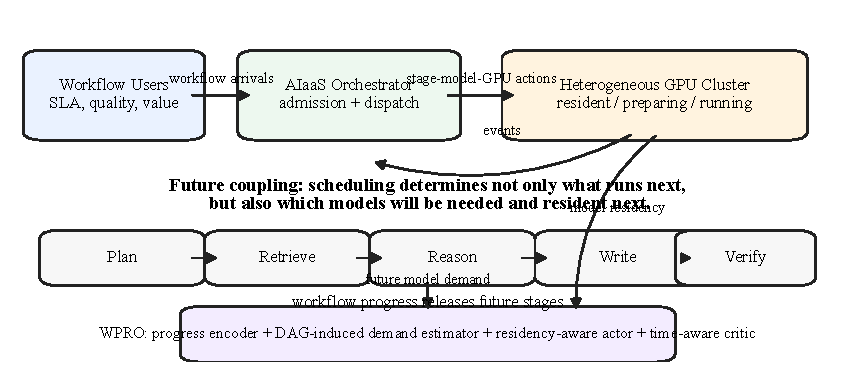
\includegraphics[width=\linewidth]{Figures/fig_system_future_coupling.pdf}
    \caption{Future coupling in agentic LLM orchestration. Completing stages changes future ready sets, while model selection changes GPU residency and future model-preparation latency.}
    \label{fig:future_coupling}
\end{figure}

\section{Related Work}

\textbf{Agentic LLM workflows.}
Foundation models \cite{brown2020language,bommasani2021foundation}, instruction tuning \cite{ouyang2022training}, and frontier LLMs \cite{openai2023gpt4} enable AI services that perform multi-step reasoning and tool use. Chain-of-thought and tree-of-thought methods elicit structured reasoning \cite{wei2022chain,yao2024tree}; ReAct, Toolformer, Reflexion, AutoGen, SWE-agent, and communicative software agents demonstrate tool-using and multi-agent workflows \cite{yao2023react,schick2023toolformer,shinn2023reflexion,wu2023autogen,yang2024sweagent,qian2024communicative}. These works motivate workflow-centric serving, but they do not solve the platform-level orchestration problem.

\textbf{LLM serving systems.}
vLLM improves KV-cache memory management with PagedAttention \cite{kwon2023vllm}. Orca schedules generative inference at iteration granularity \cite{yu2022orca}. Sarathi-Serve, DistServe, and Splitwise improve prefill/decode execution \cite{agrawal2024sarathi,zhong2024distserve,patel2024splitwise}. FlashAttention, efficient transformer inference, FlexGen, DeepSpeed-Inference, and speculative inference improve attention, memory, and decoding efficiency \cite{dao2022flashattention,pope2023efficiently,sheng2023flexgen,aminabadi2022deepspeed,miao2023specinfer}. These systems are complementary to \WPRO: they optimize how a selected model executes tokens, while \WPRO\ decides which workflow stage, model, and GPU should be selected under future workflow/residency coupling.

\textbf{Multi-model and residency-aware serving.}
S-LoRA and Punica support many concurrent LoRA adapters \cite{sheng2023slora,chen2023punica}; Llumnix studies dynamic scheduling for LLM serving \cite{sun2024llumnix}. These works recognize memory and residency as first-class serving concerns. \WPRO\ differs by connecting residency to workflow progress: keeping or replacing a resident model is evaluated according to the future model demand induced by unfinished DAGs.

\textbf{Workflow, cluster, and RL scheduling.}
HEFT and EDF are classical task and deadline scheduling methods \cite{topcuoglu2002heft,liu1973scheduling}. Sparrow, Firmament, Tiresias, and Gandiva schedule distributed and GPU clusters \cite{ousterhout2013sparrow,gog2016firmament,gu2019tiresias,xiao2018gandiva}. DeepRM and Decima learn scheduling policies with reinforcement learning \cite{mao2016deeprm,mao2019decima}. Actor--critic, GAE, PPO, and SMDP theory provide general foundations \cite{mnih2016asynchronous,schulman2016gae,schulman2017ppo,puterman1994mdp,sutton2018reinforcement}. \WPRO\ uses these foundations but introduces orchestration-specific state, action, and value structure.

\section{Modeling and Formulation}

\subsection{System Overview}

The system contains two entities: workflow users and an AIaaS platform. Users continuously submit agentic workflow requests with latency and quality requirements. The platform contains a workflow orchestrator and a heterogeneous GPU serving cluster. The orchestrator maintains active workflows, arrival buffers, ready stages, tool events, model residency, and GPU state. The GPU cluster executes LLM stages using heterogeneous foundation models.

The workflow lifecycle is event-driven. First, a user submits a workflow request. Second, the platform makes an admission decision according to capacity and SLA feasibility. Third, dependency-ready tool stages are automatically launched, while ready LLM stages enter the GPU scheduling set. Fourth, at each orchestration event, the orchestrator jointly selects workflow stage, model, and GPU assignments. Finally, stage completions update workflow progress, communication delays determine successor release times, and the selected model becomes resident after preparation/execution.

\subsection{Workflow, Model, and GPU State}

Workflow \(j\) is a DAG \(G_j=(\calV_j,\calE_j)\). Stage \(i\in\calV_j\) has semantic type \(q_{ji}\), execution class \(c_{ji}\in\{\textsf{llm},\textsf{tool},\textsf{comm}\}\), input tokens \(N^{\mathrm{in}}_{ji}\), output tokens \(N^{\mathrm{out}}_{ji}\), and output size \(s_{ji}\). Workflow \(j\) arrives at \(a_j\), has deadline \(D_j\), and weight \(w_j\).

At event \(k\) and time \(t_k\), the system state is
\begin{equation}
S_k=\left(\calW_k,\calR_k,\calG_k,\calM_k,t_k\right),
\end{equation}
where \(\calW_k\) is the active workflow set, \(\calR_k\) is the ready LLM-stage set, \(\calG_k\) is the GPU state, and \(\calM_k\) is the model-residency state. GPU \(g\) has memory capacity \(B_g\), server location, speed profile, resident model \(\rho_g(t_k)\), target model under preparation \(\tilde\rho_g(t_k)\), and running stage state.

A stage \((j,i)\) is ready when all predecessors complete and communication delay has elapsed:
\begin{equation}
(j,i)\in\calR_k \Leftrightarrow c_{ji}=\textsf{llm},~
\mathrm{Pred}_j(i)\subseteq C_j(t_k),~r_{ji}\le t_k,
\end{equation}
where \(C_j(t_k)\) is the completed-stage set and \(r_{ji}\) is the stage release time.

\subsection{Latency and Residency}

Model preparation latency depends on residency:
\begin{equation}
L^{\mathrm{prep}}_{g,m}(t)=
\begin{cases}
0, & \rho_g(t)=m,\\
L^{\mathrm{adp}}_{g,m}, & m \text{ is adapter-compatible},\\
L^{\mathrm{load}}_{g,m}, & \text{otherwise}.
\end{cases}
\end{equation}
Expected LLM execution latency is token-dependent:
\begin{equation}
\bar L^{\mathrm{exec}}_{ji,m,g}=
\alpha_{m,g}N^{\mathrm{in}}_{ji}+\beta_{m,g}N^{\mathrm{out}}_{ji}
\chi_{q_{ji},m,g}.
\end{equation}
The simulator samples actual perturbation only after a dispatch is committed:
\begin{equation}
L^{\mathrm{exec}}_{ji,m,g}=\bar L^{\mathrm{exec}}_{ji,m,g}\xi_{ji,m,g}.
\end{equation}
This avoids random-number leakage across policies during action scoring. If a predecessor stage \(i\) and successor \(i'\) are placed across servers, communication delay is
\begin{equation}
L^{\mathrm{com}}_{ji,i',g,g'}=\ell_{g,g'}+\frac{s_{ji}}{B_{g,g'}}.
\end{equation}

\subsection{Decision Variables and Objective}

At event \(k\), the orchestrator decides admission variables \(x_j\in\{0,1\}\) for newly arrived workflows and dispatch actions for idle GPUs. A dispatch action is
\begin{equation}
a_{k,g}\in
\{(j,i,m,g):(j,i)\in\calR_k,~m\in\calM_{ji},~b_m\le B_g\}
\cup\{\textsf{WAIT}_g\}.
\end{equation}
The objective is weighted SLA-compliant value:
\begin{equation}
\max_{\pi}~
\mathbb{E}_{\pi}\left[
\sum_{j} w_j \ind\{T_j-a_j\le D_j,~j\mathrm{~completed}\}
\right].
\label{eq:objective}
\end{equation}
We also report weighted goodput rate \(G_{\mathrm{w}}=V_{\mathrm{w}}/T_{\mathrm{episode}}\), admission ratio \(R_{\mathrm{adm}}\), on-time ratio \(R_{\mathrm{on}}\), P95 latency, residency hit ratio, and preparation overhead.

\subsection{Problem Characteristics}

Even a restricted offline version is NP-hard by reduction from 0--1 knapsack: one GPU, one event, independent single-stage workflows, deterministic processing times, and a common deadline reduce to selecting jobs with maximum value under a capacity budget. Online orchestration is harder because arrivals are unknown, execution times are stochastic, tool completions release new stages, and model residency makes future costs decision-dependent. Therefore, greedy matching over the current ready set cannot generally optimize \eqref{eq:objective}.

\section{Online Orchestration Design}

\subsection{Algorithmic Idea}

The event-driven process forms a semi-Markov decision process (SMDP). The Bellman recursion must account for nonuniform event intervals:
\begin{equation}
V^{\pi}(S_k)=
\mathbb{E}_{\pi}\left[
R_k+e^{-\beta\Delta t_k}V^{\pi}(S_{k+1})\mid S_k
\right].
\end{equation}
\WPRO\ approximates this long-term value with a structured actor--critic architecture.

\subsection{Workflow-Progress Representation}

For each active workflow, \WPRO\ encodes completed-stage ratio, ready-stage ratio, remaining critical path, successor-stage types, deadline slack, ready waiting time, and service-class weight. Let \(h_j=f_{\theta}^{\mathrm{wf}}(W_j)\). Active workflows are aggregated with a permutation-invariant pooling operator:
\begin{equation}
h_{\mathrm{W}}=\mathrm{Pool}\{h_j:j\in\calW_k\}.
\end{equation}
GPU states are encoded similarly into \(h_{\mathrm{G}}\). The global embedding is \(h_k=[h_{\mathrm{W}},h_{\mathrm{G}},h_{\mathrm{sys}}]\).

\subsection{Future Model-Demand Prediction}

For each model \(m\), \WPRO\ estimates the near-future demand induced by unfinished DAGs:
\begin{equation}
\hat d_m(H\mid S_k)=f_{\psi}^{\mathrm{dem}}(h_k,m).
\end{equation}
The auxiliary target \(d_m^{\mathrm{DAG}}(H\mid S_k)\) is computed from current unfinished workflows, estimated release times, slack, and feasible models. It is not a perfect future trace oracle; it is a DAG-induced model-demand label. The loss is
\begin{equation}
\mathcal{L}_{\mathrm{dem}}=\sum_{m\in\calM}
\left(\hat d_m(H\mid S_k)-d_m^{\mathrm{DAG}}(H\mid S_k)\right)^2.
\end{equation}

\subsection{Residency-Aware Joint Action Representation}

For a candidate \(a=(j,i,m,g)\), \WPRO\ constructs an action-specific vector
\begin{equation}
\phia(S_k,a)=[h_k,h_j,h_i,h_m,h_g,h_{\mathrm{cross}}],
\end{equation}
where \(h_{\mathrm{cross}}\) includes slack, remaining critical path, preparation time, expected execution time, resident hit, adapter compatibility, target-model demand \(\hat d_m(H)\), and evicted-model demand \(\hat d_{\rho_g}(H)\). The structural residency term is
\begin{equation}
\Delta\Psi_{j,i,m,g}=
\hat d_m(H)-\hat d_{\rho_g}(H)-\lambda L^{\mathrm{prep}}_{g,m}.
\end{equation}
The actor logit is
\begin{equation}
\ell_{\theta}(S_k,a)=\theta^\top\phia(S_k,a)+\eta\Delta\Psi_{j,i,m,g}.
\end{equation}
Because logits depend on action-specific features, the actor can learn relative preferences among candidates at the same event.

\subsection{Hierarchical Autoregressive Policy}

Directly enumerating all dispatch matrices is infeasible. \WPRO\ decomposes one event into a hierarchical autoregressive matching process:
\begin{equation}
\pi_{\theta}(A_k\mid S_k)=
\prod_{g\in\calI_k}
\pi_{\theta}(a_{k,g}\mid S_k,a_{k,<g}).
\end{equation}
After assigning one GPU, the selected stage is removed, feasibility masks are updated, and the next GPU is processed. The action set also includes \(\textsf{WAIT}\), allowing the policy to preserve useful residency until the next exogenous event.

\begin{algorithm}[t]
\caption{\WPRO\ at an orchestration event}
\label{alg:wpro}
\begin{algorithmic}[1]
\State Observe \(S_k=(\calW_k,\calR_k,\calG_k,\calM_k,t_k)\)
\State Encode workflow progress and GPU residency
\State Estimate \(\hat d_m(H\mid S_k)\) for all \(m\in\calM\)
\State Initialize dispatch set \(A_k\gets\emptyset\)
\For{idle GPU \(g\in\calI_k\)}
    \State Build feasible candidates plus \(\textsf{WAIT}_g\)
    \State Score each candidate by action-specific features
    \State Select \(a_{k,g}\sim\pi_{\theta}(\cdot\mid S_k,a_{k,<g})\)
    \State Update masks and temporary residency state
\EndFor
\State Execute \(A_k\), observe \(R_k,\Delta t_k,S_{k+1}\)
\State Store SMDP transition for actor--critic training
\end{algorithmic}
\end{algorithm}

\subsection{Time-Aware Actor--Critic Learning}

The TD residual is
\begin{equation}
\delta_k=R_k+e^{-\beta\Delta t_k}V_{\phi}(S_{k+1})-V_{\phi}(S_k).
\end{equation}
Time-aware GAE is
\begin{equation}
\hat A_k=\sum_{\ell\ge0}
\left(\prod_{r=0}^{\ell-1}e^{-\beta\Delta t_{k+r}}\lambda_{\mathrm{GAE}}\right)
\delta_{k+\ell}.
\end{equation}
The softmax policy gradient uses
\begin{equation}
\nabla_\theta\log\pi_\theta(a\mid S)=
\phia(S,a)-\sum_{a'}\pi_\theta(a'\mid S)\phia(S,a').
\end{equation}
Thus the actor learns dispatch preferences over workflow--stage--model--GPU candidates rather than shifting all logits by a state-only constant.

\section{Theoretical Analysis}

\textbf{Feasibility.}
The autoregressive decoder enforces feasibility by construction. At each substep, the candidate mask includes only ready LLM stages, feasible models, GPUs with sufficient memory, and stages not already selected in the current event. Tool stages are handled by exogenous tool-completion events and never consume GPU dispatch capacity.

\textbf{Complexity.}
Let \(G_I=|\calI_k|\), \(R=|\calR_k|\), \(M_{\max}\) be the maximum feasible models per stage, and \(F\) be feature dimension. A direct dispatch-matrix enumeration is exponential in \(G_I\). \WPRO\ evaluates at most \(O(G_I R M_{\max})\) candidate actions per event, with scoring cost \(O(F)\) per candidate.

\textbf{Policy invariance of shaping.}
The potential term uses the same event discount \(e^{-\beta\Delta t_k}\) as the SMDP return. Therefore, potential-based shaping changes learning signals but preserves optimal policies under the standard potential-shaping argument. The chosen potential increases with workflow progress and decreases when slack is consumed without progress, avoiding positive reward for pure waiting.

\section{Performance Evaluation}

\subsection{Experimental Setup}

We implement a trace-driven event simulator. Workflows are generated from agentic templates including research, coding, and document-analysis DAGs, and public LLM-serving traces such as BurstGPT can be used to drive arrivals and token lengths \cite{wang2024burstgpt}. Stage classes are separated into LLM, tool, and communication stages. Models represent heterogeneous planning, reasoning, retrieval, generation, and verification capabilities. GPUs differ in memory, speed, and server location. Execution time depends on input/output tokens, model/GPU rates, semantic stage type, and sampled perturbation. Model residency follows resident--preparing--running states.

Trace-driven experiments use chronological train/validation/test separation. The first 60\% of the trace is used for training, the next 20\% for validation checkpoint selection, and the final 20\% for held-out testing, with guard intervals around split boundaries. Each final configuration should use five independent RL training seeds, at least twenty paired test windows, bootstrap 95\% confidence intervals, and Wilcoxon signed-rank tests against the strongest online baseline.

\subsection{Baselines and Metrics}

We compare against FCFS, EDF, SRPT, Utility-Greedy, Lyapunov, DAG-Oracle Greedy, Vanilla A2C, PPO, and adapted vLLM/Orca/Sarathi-style queueing policies under the same simulator. DAG-Oracle Greedy can access \(d_m^{\mathrm{DAG}}(H)\), so it is labeled as an oracle heuristic rather than a deployable online policy. Metrics include \(V_{\mathrm{w}}\), \(G_{\mathrm{w}}\), \(R_{\mathrm{adm}}\), \(R_{\mathrm{on}}\), conditional SLA success, P95 latency, residency hit ratio, preparation time, communication overhead, queue waiting, demand-prediction error, and decision overhead.

\begin{table}[t]
\centering
\caption{Unified baseline adaptation.}
\label{tab:baselines}
\begin{tabular}{lll}
\toprule
Method & Main signal & Future/residency awareness \\
\midrule
FCFS/SRPT/EDF & queue order & no \\
Utility-Greedy & slack, prep, exec & myopic only \\
Lyapunov & queue drift & limited \\
DAG-Oracle Greedy & DAG demand label & oracle heuristic \\
Vanilla A2C/PPO & learned snapshot & no WPRO modules \\
\WPRO & progress + demand + residency & yes \\
\bottomrule
\end{tabular}
\end{table}

\subsection{Overall Performance}

Fig.~\ref{fig:overall} reports the primary service-level metrics. \WPRO\ improves normalized utility and on-time completion, while its admission ratio remains deliberately controlled. This is important: the objective is not to maximize the number of admitted workflows, but to admit and orchestrate workflows that can finish before deadline with high weighted value.

\begin{figure*}[t]
\centering
\subfloat[Weighted utility]{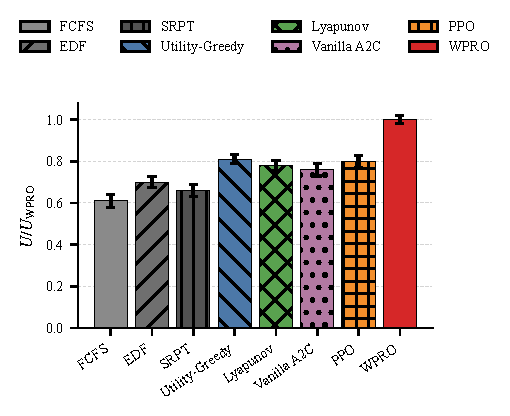
\includegraphics[width=0.315\linewidth]{Figures/split/fig_overall_utility.pdf}}
\hfill
\subfloat[Admission ratio]{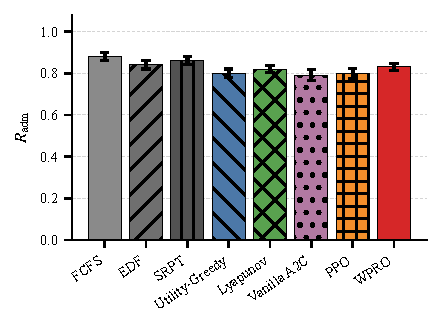
\includegraphics[width=0.315\linewidth]{Figures/split/fig_overall_admission.pdf}}
\hfill
\subfloat[On-time ratio]{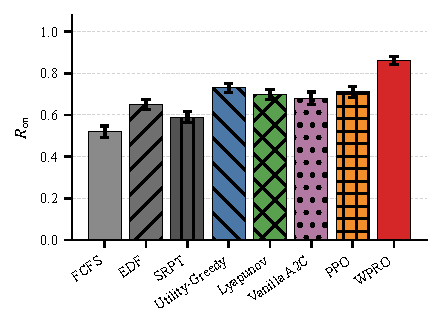
\includegraphics[width=0.315\linewidth]{Figures/split/fig_overall_ontime.pdf}}
\caption{Overall performance under the unified simulator. Each panel is generated independently and composed in LaTeX to avoid legend/text overlap. Error bars denote 95\% confidence intervals over paired test windows.}
\label{fig:overall}
\end{figure*}

\subsection{Scalability and Robustness}

Fig.~\ref{fig:scale} varies arrival rate \(\lambda\). Under light load, several policies can recover from suboptimal residency choices because GPUs have enough slack. Under heavy load, cold-load mistakes and poor future-stage anticipation accumulate. \WPRO\ maintains higher utility and on-time completion by preserving useful resident models and prioritizing workflows whose downstream demand is imminent.

\begin{figure*}[t]
\centering
\subfloat[Weighted utility]{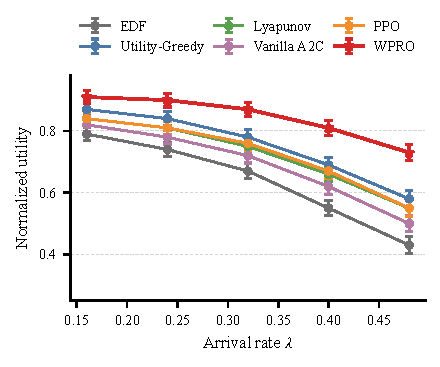
\includegraphics[width=0.315\linewidth]{Figures/split/fig_scale_utility.pdf}}
\hfill
\subfloat[On-time ratio]{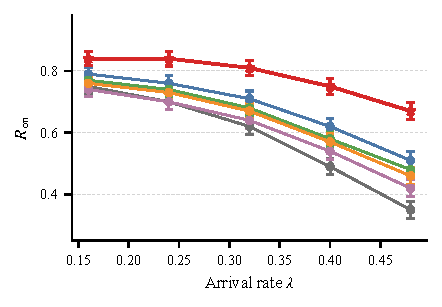
\includegraphics[width=0.315\linewidth]{Figures/split/fig_scale_ontime.pdf}}
\hfill
\subfloat[Admission ratio]{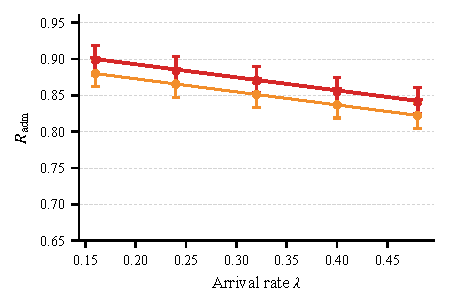
\includegraphics[width=0.315\linewidth]{Figures/split/fig_scale_admission.pdf}}
\caption{Scalability with arrival rate. The advantage of future-aware orchestration grows as workload pressure increases.}
\label{fig:scale}
\end{figure*}

Fig.~\ref{fig:robust_breakdown} further evaluates robustness and latency composition. The scatter plot compares \WPRO\ against the strongest baseline in each setting; points above \(y=x\) indicate improvement. The latency breakdown shows that \WPRO's gain mainly comes from reducing queue waiting and model preparation, not from artificially reducing unavoidable token execution time.

\begin{figure*}[t]
\centering
\subfloat[Multi-environment robustness]{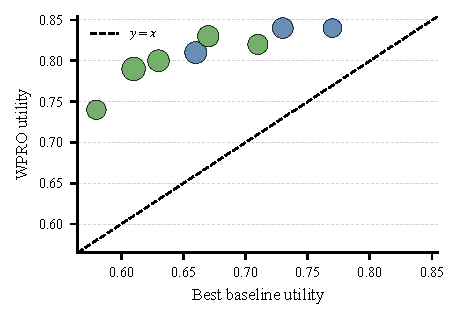
\includegraphics[width=0.46\linewidth]{Figures/split/fig_robustness_scatter.pdf}}
\hfill
\subfloat[Latency breakdown]{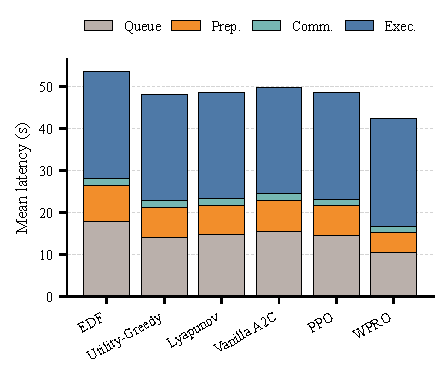
\includegraphics[width=0.46\linewidth]{Figures/split/fig_latency_breakdown_split.pdf}}
\caption{Robustness and latency analysis. \WPRO\ improves over the strongest baseline across settings and reduces orchestration-induced waiting and preparation overhead.}
\label{fig:robust_breakdown}
\end{figure*}

\subsection{Mechanism and Ablation}

Fig.~\ref{fig:mechanism} examines the two mechanisms behind the performance gain. The demand estimator tracks the DAG-induced future model-demand label \(d_m^{\mathrm{DAG}}(H)\), and the resulting demand awareness improves residency-hit ratio as load increases. This supports the core claim that workflow progress contains useful information about future model pressure.

\begin{figure*}[t]
\centering
\subfloat[DAG-induced demand estimation]{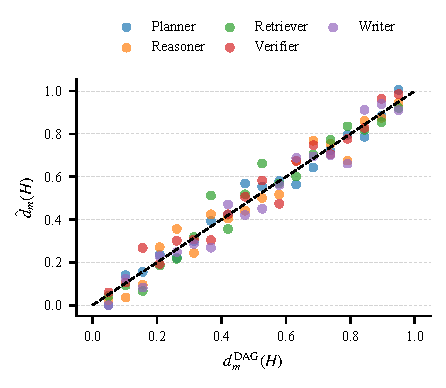
\includegraphics[width=0.46\linewidth]{Figures/split/fig_mech_prediction.pdf}}
\hfill
\subfloat[Residency hit ratio]{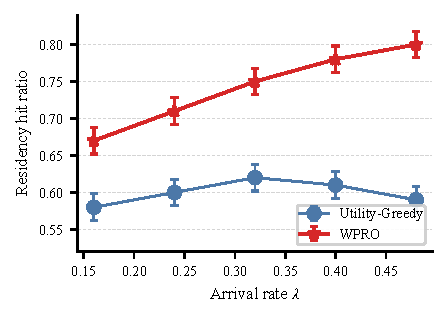
\includegraphics[width=0.46\linewidth]{Figures/split/fig_mech_residency.pdf}}
\caption{Mechanism analysis. \WPRO\ estimates near-future model demand induced by unfinished DAGs and translates it into better residency preservation.}
\label{fig:mechanism}
\end{figure*}

Fig.~\ref{fig:ablation} removes major modules from \WPRO. Removing future-demand estimation weakens anticipation of downstream model pressure. Removing residency features weakens model-retention decisions. Removing progress representation loses information about unfinished DAG structure. Removing WAIT or shaping primarily affects deadline-pressure behavior and training stability.

\begin{figure*}[t]
\centering
\subfloat[Weighted utility]{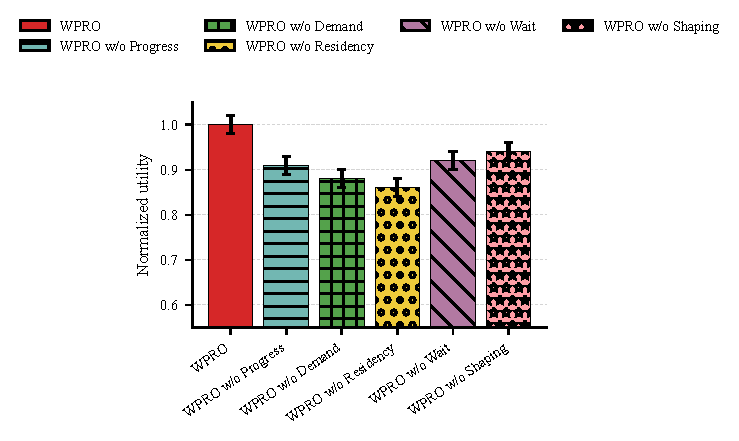
\includegraphics[width=0.315\linewidth]{Figures/split/fig_ablation_utility.pdf}}
\hfill
\subfloat[On-time ratio]{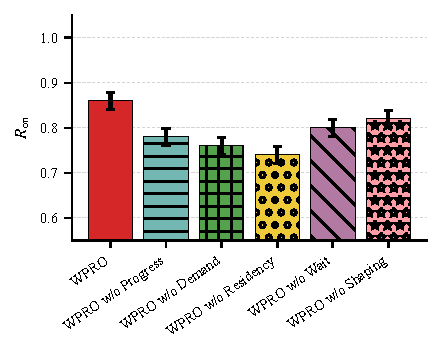
\includegraphics[width=0.315\linewidth]{Figures/split/fig_ablation_ontime.pdf}}
\hfill
\subfloat[Residency hit]{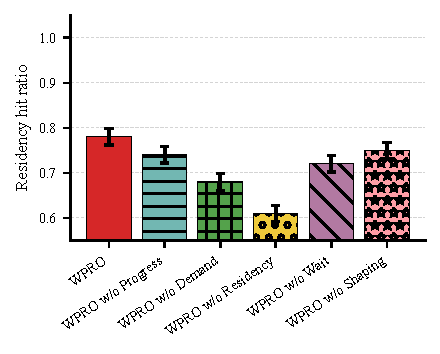
\includegraphics[width=0.315\linewidth]{Figures/split/fig_ablation_residency.pdf}}
\caption{Ablation study. Each structural component contributes to either long-term utility, deadline satisfaction, or residency efficiency.}
\label{fig:ablation}
\end{figure*}

\subsection{Scheduling Behavior and Overhead}

Fig.~\ref{fig:behavior} visualizes scheduling behavior and decision cost. The timeline shows that \WPRO\ avoids unnecessary cold loads by exploiting resident hits when future demand is high. The overhead curve shows that the autoregressive decoder scales smoothly with the number of candidate actions because it evaluates feasible candidates sequentially rather than enumerating a full dispatch matrix.

\begin{figure*}[t]
\centering
\subfloat[Event timeline]{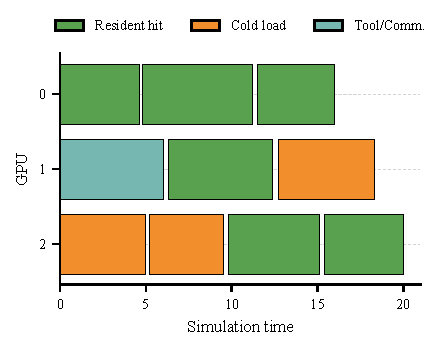
\includegraphics[width=0.46\linewidth]{Figures/split/fig_behavior_timeline.pdf}}
\hfill
\subfloat[Decision overhead]{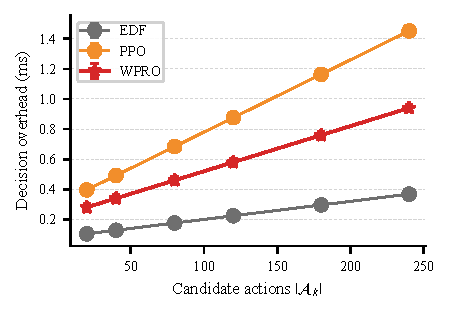
\includegraphics[width=0.46\linewidth]{Figures/split/fig_behavior_overhead.pdf}}
\caption{Scheduling behavior and runtime overhead. \WPRO\ preserves useful residency while keeping decision overhead low.}
\label{fig:behavior}
\end{figure*}

\section{Discussion}

\textbf{Relationship to LLM serving systems.}
\WPRO\ is not a replacement for vLLM, Orca, or Sarathi-Serve. Those systems optimize token execution once requests are assigned to serving replicas. \WPRO\ operates above them as a workflow-level orchestrator. Therefore, adapted baselines should be clearly described as runtime-inspired policies under a unified simulator unless the full runtime is integrated.

\textbf{Demand-prediction scope.}
\WPRO\ estimates DAG-induced near-future model demand from active workflows. It does not claim perfect prediction of unknown future arrivals. This distinction is important for a realistic paper claim and makes the auxiliary task defensible.

\textbf{Limitations.}
The current simulator models conditional repair behavior through sampled workflow templates rather than arbitrary online branching. Strict optimality gaps require CP-SAT/MILP or complete enumeration on small instances; bounded lookahead should be reported only as a reference. Future work can integrate \WPRO\ with production LLM runtimes and richer tool-outcome uncertainty.

\section{Conclusion}

We studied future-aware online orchestration for agentic LLM workflows. The key insight is that workflow scheduling and model residency are coupled: executing a stage releases future stages, while model selection changes future preparation latency. \WPRO\ captures this coupling with workflow-progress representation, DAG-induced future demand estimation, residency-aware action scoring, hierarchical autoregressive dispatch, WAIT decisions, and time-aware actor--critic learning. The resulting framework provides a principled path for AIaaS platforms to optimize weighted SLA-compliant goodput under realistic workflow, model, and GPU constraints.

\bibliographystyle{IEEEtran}
\bibliography{references}

\end{document}
